\textbf{Model uczony na stałej krzywiźnie wierzechołków}

\begin{figure}[ht]
	\centering
	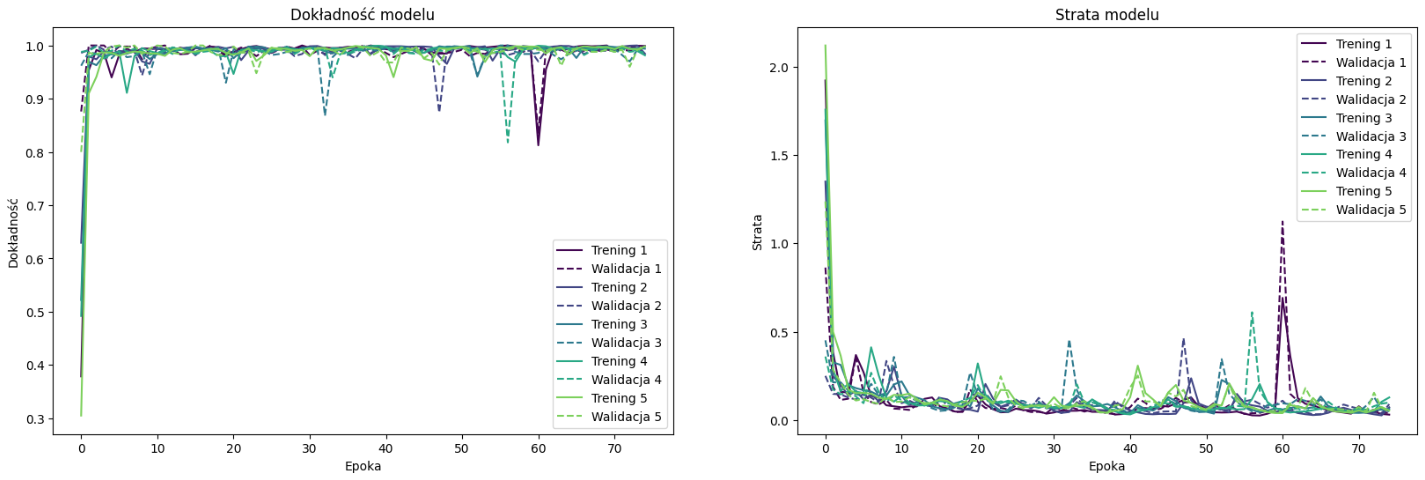
\includegraphics[height=5.5cm]{resources/tests/images/v2/multiple_edges_crossvalid_img.png}
	\caption{Wyniki testów dla modelu ze zmienną liczbą wierzchołków i walidacją krzyżową oraz stałą krzywizną wierzchołków}
	\label{Fig:tests-csvar-1}
\end{figure}
\FloatBarrier

\begin{figure}[ht]
	\centering
	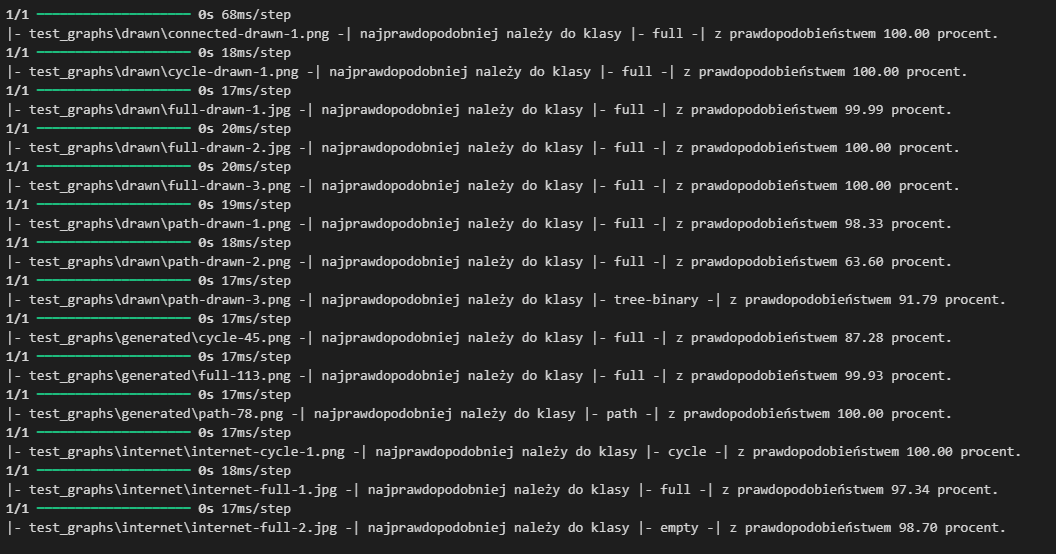
\includegraphics[height=5.5cm]{resources/tests/images/v2/multiple_edges_crossvalid_txt.png}
	\caption{Klasyfikacja obrazów zewnętrznych dla modelu ze zmienną liczbą wierzchołków i walidacją krzyżową oraz stałą krzywizną wierzchołków}
	\label{Fig:tests-csvar-2}
\end{figure}
\FloatBarrier

\textbf{Model uczony na losowej krzywiźnie wierzechołków}

\begin{figure}[ht]
	\centering
	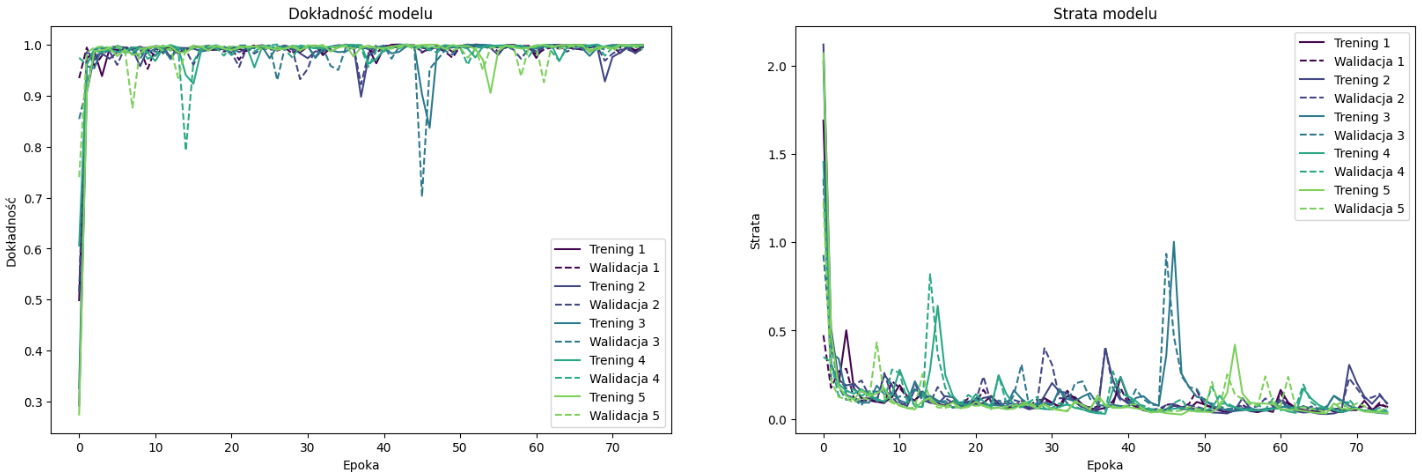
\includegraphics[height=5.5cm]{resources/tests/images/v3/multiple_edges_crossvalid_img.png}
	\caption{Wyniki testów dla modelu ze zmienną liczbą wierzchołków i walidacją krzyżową oraz losową krzywizną wierzchołków}
	\label{Fig:tests-csvar-1}
\end{figure}
\FloatBarrier

\begin{figure}[ht]
	\centering
	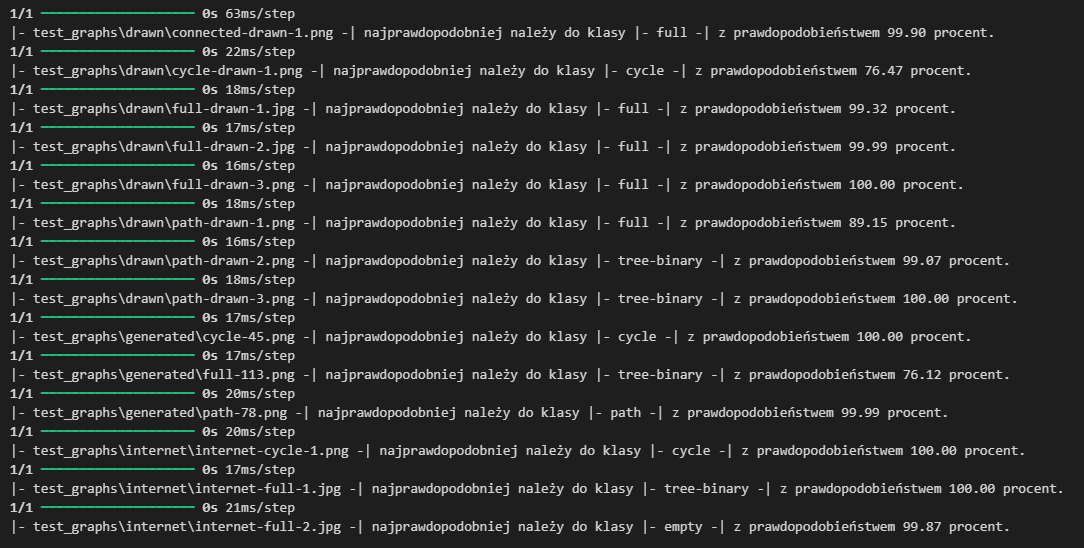
\includegraphics[height=5.5cm]{resources/tests/images/v3/multiple_edges_crossvalid_txt.png}
	\caption{Klasyfikacja obrazów zewnętrznych dla modelu ze zmienną liczbą wierzchołków i walidacją krzyżową oraz losową krzywizną wierzchołków}
	\label{Fig:tests-csvar-2}
\end{figure}
\FloatBarrier